\chapter{eXpressive Internet Architecture}
\label{chap:ccnxia}

The most common theme observed in the future Internet research is to
move away from the host centric Internet. Computers communicating to
one another was a cornerstone of the time when the Internet was
born. Therefore, the IPv4 network on which the Internet was based
addressed hosts in the network in order to establish communication
between them. Thus, the Internet as we see today has evolved on the
host based paradigm.

But, for the Internet users today it does not matter \emph{who} serves
the information. The users care about \emph{what} information they
receive. This shift of the Internet usage has given rise to a new
approach to evolve the Internet to a network infrastructure in which
focal point is the \emph{content} rather than \emph{hosts}. This
approach is generally referred to as Information Centric
Networking. \ref{fig:icn_illustration} shows an illustration of
Internet usage in information-centric Internet vs today's host-centric
Internet compared. An example of a proposed Information centric
networking architecture is Named Data Networking(NDN).

\begin{figure}
  \begin{center}
    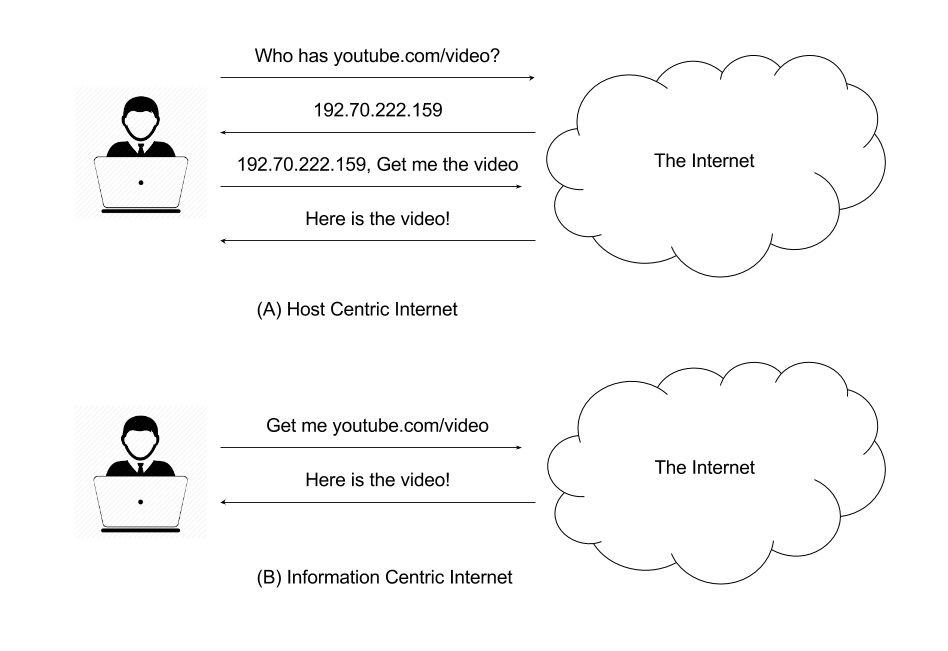
\includegraphics[scale = 0.5]{icn_illustration}
    \caption{Host Centric Internet vs Information Centric Internet}
    \label{fig:icn_illustration}
  \end{center}
\end{figure}

\section{eXpressive Internet Architecture (XIA)}
eXpressive Internet Architecture is a candidate future Internet
architecture that argues against elevating one particular
communication \emph{principal} type over others. A principal is a
named entity such as a host, a domain, a service or a specific content
piece. If the network primarily supports communication with one
particular principal type then communication with the other principal
type inherently becomes difficult. We see in today's host-centric
Internet that all the content requests first need to identify the host
who is capable of serving the content request. Similarly, if we moved
to an Information Centric Internet, it is not obvious how can we make
hosts communicate with each other. XIA, thus, supports coexistence of
multiple principal types.

Three key features of XIA are as follows:
\begin{itemize}
\item{Multiple Principal Types}
\item{Fallbacks}
\item{Intrinsic Security}
\end{itemize}
Let's go over these features one by one in order to understand XIA
better.
\subsection{Multiple Principal Types}
As seen above, XIA supports coexistence of multiple communication
principal types. The communication principals that XIA supports are
hosts, services, administrative domains and content. These principals
are identified by unique eXpressive identifiers called as
XIDs. Corresponding to the four principal types mentioned above, their
XIDs are referred to as HIDs, SIDs, ADs and CIDs.

\subsection{Intrinsic Security}
XIA's intrinsic security requirement mandates a communicating
principal to prove itself. In other words, it should be possible for
an entity that is communicating with a principal to verify the
authenticity and integrity of the principal. XIA, thus, chooses the
XID as such that they guarantee the authenticity and integrity of the
communicating principal. For example, the host identifier or the HID
is the secure hash of the host's public key. The content identifier or
the CID is the secure hash of the content itself.

\subsection{Fallbacks}
In order to support evolvibility, it becomes important to address the
issue of how network entities that do \emph{not} understand a
communication principal type deal with the principal. An analogous
example in today's Internet could be as follows. If we move to IPv6
Internet, what if an intermediate network does not understand IPv6 and
only understands IPv4? The intermediate nodes should not drop the IPv6
packets. In other words, the network still needs a way to forward
packets even if it does not understand a communication principal. XIA
supports this ability via the notion of fallbacks. Fallbacks allow XIA
to specify multiple paths to the same principal. The entities that do
not understand a particular path can take a different path for
communicating with the principal type. All the different paths to the
communication principal are combined into a network layer address that
takes the format of a directed acyclic graph (DAG) as shown in
\ref{fig:dag_address}. The address is interpreted as follows - forward
/ route primarily based on CID, but if you don't understand CID, route
based on IP address.

\begin{figure}
  \begin{center}
    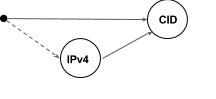
\includegraphics[scale = 0.75]{dag-cid-ipv4}
    \caption{Fallbacks}
    \label{fig:dag_address}
  \end{center}
\end{figure}

\section{Content Principal in XIA}
With the content principal users can express interest in content
irrespective of its location. Sending a content request fetches
content from anywhere in the network. The request could go all the way
back to the original publisher of the content or can be served from an
in-network cache that holds a copy of the content. The API for content
principal are as shown in table \ref{tab:cid_api}. Content principal
provides intrinsic security guarantees by choosing the cryptographic
hash of the content as its identifier. Thus, all the network devices
can verify authenticity of the content objects.

\begin{table}
  \begin{center}
    \begin{tabular}
      { l  p{3in} }
      Function & Description \\
      \hline
      getContent(socket, addr, buffer) & Retrieves the content specified
      by addr from network; addr contains CID and possibly a fallback \\
      putContent(socket, content) & Registers the content as
      available \\
      \hline
    \end{tabular}
    \caption{API for Content Principal}
  \end{center}
  \label{tab:cid_apis}
\end{table}

\section{Conclusion}
In this chapter, we studied the eXpressive Internet Architecture. We
looked at the importation features offered by XIA - coexistence of
multiple principal types, intrinsic security and fallbacks. Then we
looked at how network entities can use the content principal to
publish and fetch content irrespective of its physical location. This
was the last introductory chapter in the thesis. The following
chapters build on to ideas discussed in these two chapters and are the
main contributions of the thesis.
